\section{Methodology}

% \textbf{Methods:} We collected an in-house dataset comprising 24 laparoscopic surgery videos, each approximately 3 minutes long in 1920x1080 resolution, totalling 1.32GB. These videos feature procedures performed by either a trainee or an expert trainer. The dataset includes 103,629 frames annotated with tooltips and six degrees of freedom ground truth data for three-dimensional tool positions and quaternions for spatial rotation, with complete bounding box annotations for tools and tooltips. Multiple anchor-based and anchor-free deep learning models are implemented and tested, including various state-of-the-art (SOTA) models. These models are evaluated using the standard Common Objects in Context (COCO) metric, yielding mean Average Precision (mAP) scores for detected bounding boxes around the tools and tooltips at a 0.5 intersection over union (IoU) threshold. The models are trained on a single NVIDIA GeForce RTX 3060 GPU with 12GB of GPU memory.

\subsection{Datasets}

% rationale behind data

\subsubsection{Data Collection}

% why collecting this dataset?
% Higher POV, more detail about surgeons, more tools, higher quality of data, use in LMICs and training networks

% Data was collected on 11th and 12th October 2023 (at the 8th Urology Boot Camp).
% We collected data about the handedness and level of expertise of the participants (but not gone through any of this yet as we hadn't touched the skill side).
% Sensors were three NDI Aurora 6DoF electromagnetic trackers (one on each tools one on the camera), the calibrated position was to the fulcrum of each tool (performed by pivot calibration).
% 24 particpants with information on the usage of their hands using the Edinburgh Handedness survey \cite{oldfield_assessment_1971} in various other tasks, including writing, drawing, throwing, scissors, toothbrush, knife (without fork), spoon, broom (upper hand), striking a match (hand holding match) and opening a lid (hand opening lid).
% We also collected data on the surgeons' estimated number of procedures in their lifetimes' and within the last 12 months.
% We will confirm that the patients do not have a pacemaker or any other metal implants that could interfere with the electromagnetic tracking system.

% Use reference (See Figure 1 \ref{fig:teaser}) the black sensor on the right of the peg transfer board with the blue tap to localise the tooltips and cameras positions and orientations.
% DIAGRAM Data Collection

% Collected motion data from a peg transfer task. The goal is that we can train an AI system to localise the laparoscopic tools using the image alone. This will well help us develop a new training system, giving automated feedback on indiidual sub-skills. In this study we focus on first detecting the tools which can then be used with the sensor data to build a model which can predict the motion of the tools based on the location of the tool in the image.

% Exact dates the dataset was collected
% All information about participants available to share and discuss
% The sensor recording equipment and how it worked
% Any extra information regarding the setup or configuration

\begin{figure}
    \centering
    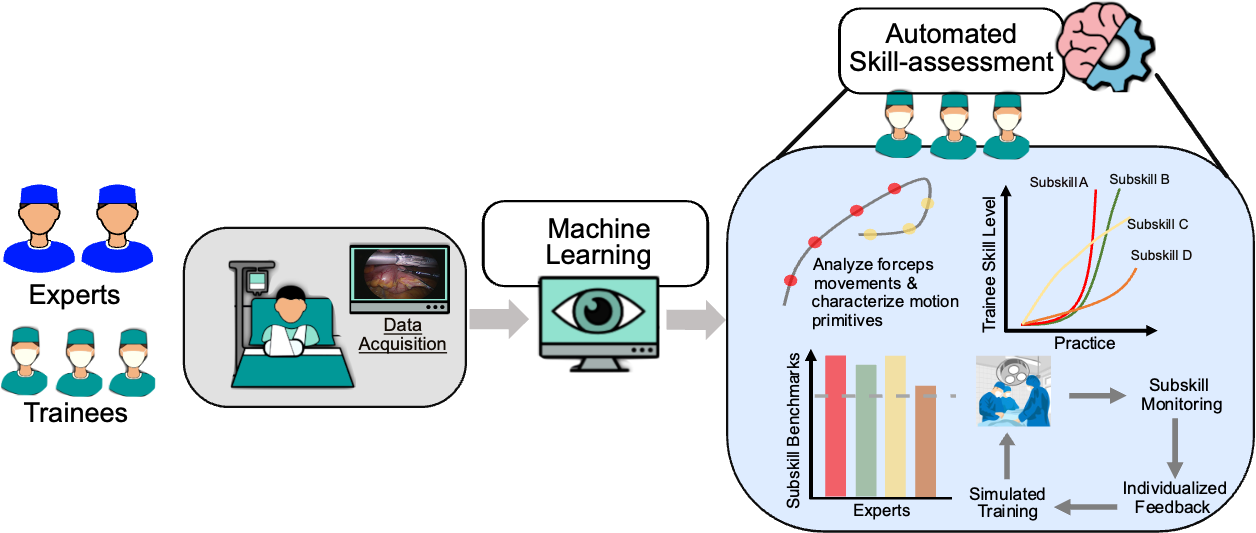
\includegraphics[width=1\linewidth]{dataset_collection.png}
    \caption{AI-Enhanced Laparoscopic Training Dataset Collection}
    \label{fig:dataset-collection}
    \Description{Handout given to surgeons preceeding the data collection process.}
\end{figure}

All participants, surgical trainees and trainers were given a handout, as shown in Figure \ref{fig:dataset-collection}, which explained the study and the data collection process. The handout explained that the study was to collect motion data from a peg transfer task. The goal was to train an AI system to localise the laparoscopic tools using the image alone. This would help develop a new training system, giving automated feedback on individual sub-skills. In this study, we focused on first detecting the tools, which could then be used with the sensor data to build a model which could predict the motion of the tools based on the location of the tool in the image.

% discuss partipants, eligibility criteria, and consent, ethics, dates of study

% specify dates of collected data - stard and end

% data collection process - cameras, sensors, images (bmp), storage

% sample size sufficiency

\subsubsection{Other Datasets}

% pre-selection of predictors and data required before model building

In the end we decided to evaluate only on the ART-Net dataset. This is because we wanted to use an existing SOTA with available models and code for reproduction and comparison. We also wanted to compare our results with the results of the ART-Net paper.

PETRAW was a dataset primarily for segmentation and workflow recognition, however we tested it for surgical tool detection and tracking. Since the dataset was collected in-situ, we have exact ground truth values. It is the gold standard for comparison of what we would want our dataset to be like in the future.

% show petraw IMAGE and example of data

% show table of different datasets, their annotations, and their use cases

\subsection{Data Preparation}

% planned outcome, how and what assessed, rationale for choosing this, consistent across all collected data, potential subjective interpretation

% quality checking

% plan for data annotation - missing data, outliers, duplicates, errors, inconsistencies, and how to handle them, using https://labelbox.com/research/

% producing in COCO format

% converting other datasets to COCO format - helper functions

% using standard CV techniques to focus on tools and filter out background. problem is they are not very robust and may not work well in all cases and highly subjective to noise.

% attempted to get x and y position using ground truth data, however there were some errors.

\subsection{Methods Overview}

% reimplement SOTA on existing datasets like ART-Net. We would have used PETRAW but the dataset was not originally purposed for object detection and tracking, so it would be difficult to compare to existing results of developed models. An idea was to take the output of any standard SOTA object detection model and implement tracking (SurgiTrack), where we can swap YOLOv7 for YOLOv10. We considered running the model on all images in the entire dataset to have reliable annotated data (though not perfect). Due to the accuracy in object detection, we can create label files in COCO format

% table showing hardware configuration, Ryzen 3900X, 32GB RAM, RTX 3060 12GB, Windows 11 Pro, PyTorch 2.2.1+cu121

\subsection{Reimplementation of the State-of-the-Art}

\subsubsection{Anchor-based Object Detection}

% rationale for choosing YOLOv10 (eliminates NMS), and ART-Net

% Backbone: Responsible for feature extraction, the backbone in YOLOv10 uses an enhanced version of CSPNet (Cross Stage Partial Network) to improve gradient flow and reduce computational redundancy.
% Neck: The neck is designed to aggregate features from different scales and passes them to the head. It includes PAN (Path Aggregation Network) layers for effective multiscale feature fusion.
% One-to-Many Head: Generates multiple predictions per object during training to provide rich supervisory signals and improve learning accuracy.
% One-to-One Head: Generates a single best prediction per object during inference to eliminate the need for NMS, thereby reducing latency and improving efficiency. 
% NMS-Free Training: Utilizes consistent dual assignments to eliminate the need for NMS, reducing inference latency.
% Holistic Model Design: Comprehensive optimization of various components from both efficiency and accuracy perspectives, including lightweight classification heads, spatial-channel decoupled down sampling, and rank-guided block design.
% Enhanced Model Capabilities: Incorporates large-kernel convolutions and partial self-attention modules to improve performance without significant computational cost.
% https://docs.ultralytics.com/models/yolov10/

% transfer learning, multiclass learning, multiloss learning - multiclass learning alabi paper

\subsubsection{Anchor-free Object Detection}

% art net paper	https://arxiv.org/pdf/2401.08256 

\subsection{Model Configuration}

\subsubsection{Object Detection}

\subsubsection{Object Tracking}

\subsection{Model Training}

There are some points to be made clear about the training processes. We will use patience set to 10, batch size of 16 but 8 in models which require more GPU memory (the SIMO models and EfficientDet). The YOLO models used a specific type of mosaic augmentation where images are cropped and stitched together to form a larger image, improving generalisation. Inference time was based on the detection times per image over the test set. The YOLOv10 models on the AI-ELT dataset were fine-tuned versions of the YOLOv10 models trained on the ART-Net dataset so epoch numbers are not completely representative. Simiarly, both RetinaNet models with anchor-based optimisation were fine-tuned versions of the non-optimised models. We also reduced the frequency of testing on validation set to every 10 epochs to reduce the time taken to train the models in this specific case. However, none of these points will take away from the main results.

% using the data and splits

% data augmentation - why, how, what, when, where, which, and how much

% hyperparameters - YOLO file

\subsubsection{Loss Functions}

% YOLO loss function

% ART-Net loss function - bounding box, confidence, and class loss

% Initially we used confidences however due to the nature of loss functions, we decided to remove them.

\subsubsection{Evaluation Metrics}

% evaluation metrics - % IoU, mAP50, mAP50-95, MSE, precision, recall

% plots and visualisations

\subsubsection{Model Updating}

% 1.	I've been training on my local PC with my 3060 (with 12gb of GPU memory). Used the ART-Net dataset with 50 epochs (took just over 4 hours). That was using the largest YOLO model with 71m params. Getting extremely high mAP and precision scores but I had a small issue with data overlap in validation and test so I need to re-run to get these values accurately (thats why i tested on other data to see if this was a serious mistake but as you'll see it doesn't look like it is).
% 2.	Results are really good for detection and segmentation on actual surgical videos. On PETRAW and our dataset it isnt very good. Plan is to scrap idea of training with EndoVis2015 and focusing on training on PETRAW, seeing what results I can get. This will also make writing the paper and evaluation much easier since we will narrow the focus so much but should also be better as I incorporate ideas from methods applied to traditional datasets. 
% 3.	I will continue to train up to 300 epochs on ARTnet for now (looked online at it seems I should continue until it overfits, some recommend even 1200 epochs) and see what final results I obtain. Then I will take the best model and use this as the basis for training on the PETRAW dataset (might as well take advantage of the data I do have - I could possible train on much more data but I will only do this if there is a severe problem). For the future I do like the idea of using the ARTnet dataset and creating classes for all other bits of data (tool tip, center and edge lines). I could always augment the data and remove background (since segmentation mask is so good) and put a random background behind of some pegs, then test on our dataset to see if it can learn this. Because of the issues in labelled datasets across the board, doing the maximum of what I can, I think, makes so much sense. I could always use the other data in the future and combine it all together in one massive dataset to try and get a SOTA if that ends up being on the cards (but I do doubt it for now, especially if the results here will be good enough).
% 4.	Only problem I see currently is that the tools look to have reflective surfaces in PETRAW. We will see if thats actually a big problem later (you can look at how it literally detects everything but the tool).
% 5.	Based on the time training is going on these kinds of models, I think I will stick to training on my local pc rather than using ARC or JADE. I feel like its the better option considering I'm not in Leeds right now and the best way to jump the learning curve is to work with the other students. After the MSc I'll probably look at working more closely with Loza and Sharib's other AIMS students. 
% 6.	Plan for tomorrow is to train on PETRAW and I'll send over some intermittent results. Then the next week or so will be looking at computer vision methods to obtain the tool tip based on segmentation mask and bounding box. Whilst Im abroad i can use remote desktop which is nice.
% 7.	Also, I got almost 500k frames in the end from training + test data of the PETRAW videos. But I only trained with a few 567 images. So overall, the full dataset will not be that useful, considering I am already getting this kind of results on that data
% 8.	I think for the PhD if we want to use our data it will have to be labelled somehow. The data is so rich and would be so powerful if we did have that extra information. 
% 9.	I have an idea to use a weakly-supervised method (which I would need to check is novel). The idea being since we have ground truth position of x and y, I can try to do some maths to get the position of x and y in the 2d image. I can run separate foreground and background by looking at colour changing pixels and take that foreground image, remove the background, and then run my model. It should easily pick up the different tools and I can make it factor in the object being picked up too (so a 2 class model). 
% 10.	From here I can check to see if the tool tip ground truth exists inside the segmentation for each respective tool and use some new appropriate metrics.
% 11.	I’m trying to think of feasibility right now and I like the idea of working on our dataset and making the most of it, rather than trying to make a SOTA on another dataset.
% 12.	The idea of labelling here was to extract the surgical workflow at the given time with very precise labels, segmentation mask for tools and the object we focus on (no need to think about the rest of the image, but segmentation would not be too difficult there). 
% 13.	Given I got a very good model using PETRAW within a few epochs and a few hundred images, it is not that difficult or infeasible to make it happen. In fact, I could begin with bounding boxes which would be so fast compared to full segmentation of the tool (but still apply segmentation if I wanted to). 
% 14.	From this labelled data, we train the model solely with our in house data and not using any other datasets since there would be no need (my results right now on combining datasets are not very promising - mAP of ~0.6). 
% 15.	Using PETRAW was my idea because of the similarities in data. I thought it would be decent when evaluated on our in house. One thing I could do is use the segmentation mask to change the colours of the entire image to something more similar of what we have. Could even adapt the tool to make it look more similar to our ones.
